\section{March 09: Basic of Foliations}

Foliations in differential geometry

\begin{definition}
  Let $M$ be a $n$-dimensional smooth manifold. 

  \begin{enumerate}
    \item A \emph{foliated chart} of dimension $r$ on $M$ is a pair $(U, \phi)$, where $U$ is an open subset of $M$ and $\phi: U \to I^r \times I^{n-r}$ is a diffeomorphism, where $I$ is the unit interval $(0, 1) \subset \bbR$.

      A \emph{plaque} of $(U, \phi)$ is a fiber of 
      \[ U \to I^r \times I^{n-r}  \xrightarrow{p_2} I^{n-r}, \]
      i.e. $\phi^{-1}(I^r \times \{y\})$ for some $y \in I^{n-r}$.

    \item A \emph{foliated atlas} of $M$ is a collection $\{(U_\alpha, \phi_\alpha)\}_{\alpha \in \Lambda}$ of foliated charts such that 
      \begin{enumerate}
        \item $\bigcup_{\alpha \in \Lambda} U_\alpha = M$,
        \item for any $\alpha, \beta \in \Lambda$, $(U_\alpha,\phi_\alpha)$ and $(U_\beta, \phi_\beta)$ are \emph{compatible}, i.e. for any plaque $P_\alpha$, $P_\beta$ of $(U_\alpha, \phi_\alpha)$ and $(U_\beta, \phi_\beta)$ respectively, $P_\alpha \cap P_\beta$ is open in both $P_\alpha$ and $P_\beta$. 
          (Note that $P_\alpha \cap P_\beta$ is also closed in $P_\alpha \cap (U_\alpha \cap U_\beta)$ and $P_\beta \cap (U_\alpha \cap U_\beta)$, hence $P_\alpha \cap P_\beta$ is a union of connected components of both $P_\alpha$ and $P_\beta$.) 
          In other words, 
            \[ \{\text{connected components of } P_\alpha \cap U_\alpha \cap U_\beta\} = \{\text{connected components of } P_\beta \cap U_\alpha \cap U_\beta\}. \]
      \end{enumerate}

    \item Two foliated atlases are \emph{equivalent} if their union is a foliated atlas. 
      A \emph{foliation} on $M$ is an equivalence class of foliated atlases on $M$.

    \item A \emph{leaf} of a foliation on $M$ is a \textbf{connected} subset $L \subset M$ which is union of at most countably many plaques such that for any plaque $P$ of any foliated chart, we have $L \cap P = \emptyset$ or $P \subset L$.
  \end{enumerate}
\end{definition}

\begin{remark}
  We have
  $M = \bigsqcup \text{leaves}$.
  Every leaf is a manifold with an ``injection'' to $M$.
\end{remark}

\begin{example}
  Let $M$, $N$ be smooth manifolds.
  A map $\pi : M \to N$ is a \emph{submersion} if for any $x \in M$, the differential $d_x \pi : T_x M \to T_{\pi(x)} N$ is surjective.
  By implicit function theorem, locally $\pi$ is diffeomorphic to the projection $I^m \to I^{m-r}$.
  Then the collection of charts of $M$ which are compatible with $\pi$ forms a foliated atlas, and hence defines a foliation on $M$.
  In this case, the leaves are the connected components of fibers of $\pi$.
\end{example}

Let $M$ be a smooth manifold, and $\calT_M$ be the sheaf of smooth vector fields on $M$.
Recall the \emph{Lie bracket} of $\calT_M$ is a map
\[ [ - , - ] : \calT_M \times \calT_M \to \calT_M, \quad [D_1, D_2] = D_1 D_2 - D_2 D_1. \]

Let $\calF \subset \calT_M$ be a locally free subsheaf of $\calT_M$ of rank $r$ such that $\calF|_x \to \calT_M|_x$ is injective for any $x \in M$.

\begin{definition}
  We say $\calF$ is \emph{involutive} if it is closed under the Lie bracket, i.e. for any open subset $U \subset M$ and any $D_1, D_2 \in \calF(U)$, we have $[D_1, D_2] \in \calF(U)$.
\end{definition}

\begin{theorem}[Frobenius]\label{thm:Frobenius}
  Let $M$ be a manifold.
  There is a canonical bijection between foliations on $M$ and involutive locally free subsheaves of $\calT_M$.
  \[ \{\text{foliations on } M\} \longleftrightarrow \{\text{involutive subbundle of } \calT_M\} \]
\end{theorem}
\begin{proof}[Idea of proof]

  (foliation $\leadsto$ involutive subbundle)
  For chart $(U , \phi)$ of $M$, we have $\pi : U \to I^r \times I^{n-r}$.
  On $I^r \times I^{n-r}$, we have the standard coordinate $x_1, ..., x_n$.
  Then $\calF(U)$ is generated by $D_i = \pi^*  \partial x_i$ for $i = 1, ..., r$.
  Glueing $\calF(U)$ for all charts $U$ gives an involutive subbundle of $\calT_M$.

  (involutive subbundle $\leadsto$ foliation)
  Let $\calF$ be an involutive subbundle of $\calT_M$.
  If $ \rank \calF = 1$, $\calF$ is locally generated by a single vector field $D$.
  From any point $x \in M$, we can construct a integral curve $L$ of $D$ passing through $x$ by solving the ODE defined by $D$.

  If $\rank \calF = r > 1$, take $r$ local generators $D_1, ..., D_r$ of $\calF$.
  Solve some linear PDE defined by $D_1, ..., D_r$ to get a local chart of $M$ which is compatible with $\calF$.
\end{proof}

\begin{remark}
  Let $\calF \subset \calT_M$ be an involutive subbundle of $\calT_M$ with a leaf $L \subset M$.
  Then the tangent bundle of $L$ is just $\calF|_L$, i.e. 
  \[ \calF|_L = \Image(\calT_L \to \calT_M|_L). \]

  Under $\phi: U \to I^r \times I^{m-r} \to I^{m-r}$ with coordinates $x_1, ..., x_n$ and $\calF(U)$ generated by $D_i = \pi^* (\partial / \partial x_i)$ for $i=1...r$, the coordinates $x_{r+1}, ..., x_m$ are annihilated by $\calF(U)$.

  Abstractly, to get $U \to I^{m-r}$, we need $C^\infty$-functions $f_1,...,f_{m-r}$ on $U$ with $p_2 = (f_1,...f_{m-r})$ and $D f_j = 0$ for all $D \in \calF$.
\end{remark}

    
\begin{example}
    
  Let $M = \bbR^2$ with coordinate $x,y$, and $D = a \partial_x + b \partial_y$ with $a,b$ nonzero constant.
  Then $D f = 0$ implies $f = b x - a y$.
  Then $f: \bbR^2 \to \bbR$ defines a foliation with leaves given by the level sets of $f$, i.e. $\{b x - a y = c\}$ for some constant $c$.
\end{example}

\begin{example}\label{eg:foliation_by_conics}
  Let $M = \bbR^2 \setminus \{0\}$ with coordinate $x,y$, and $D = a y \partial_x + b x \partial_y$ with $a$ nonzero constant.
  Let $\calF$ be the involutive subbundle of $\calT_M$ generated by $D$.
  
  How to solve $D f = 0$?
  
  Assume $L$ is a leaf.
  Then $\calT_L$ is generated by $D|_L$.
  Consider a differential $1$-form $\omega$ on $M$ such that $\langle \omega,D \rangle = 0$, here $\langle -,- \rangle$ is the natural pairing between $\calT_M$ and $\Omega^1_M$.
  Write $\omega = u d x + v d y$, then $\langle \omega, D \rangle = a y u + b x v$.
  We can take $\omega = -b x d x + a y d y$.
  Note that $\omega|_L = 0$.
  View $x,y$ as $C^\infty$-functions on $L$ by pull-back.
  View $\omega|_L = 0$ as ODE on $L$.
  Then we get $d (b x^2 - a y^2) = 0$.
  Hence $f = b x^2 - a y^2$ is a solution of $D f = 0$.

  Then $f: \bbR^2 \setminus \{0\} \to \bbR$ defines a foliation with leaves given by the level sets of $f$.
  There are two types of leaves:
  \begin{itemize}
    \item $a / b > 0$: the leaves are hyperbolas;
    \item $a / b < 0$: the leaves are ellipses.
  \end{itemize}
  See \cref{fig:foliation_by_conic}.
\end{example}

\begin{figure}
  \begin{center}
    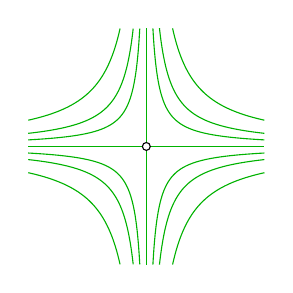
\begin{tikzpicture}[scale=0.5]
      \node[circle,inner sep = 1pt] (O) at (0,0) {};
      \draw[green!70!black] (O) -- (3,0);
      \draw[green!70!black] (O) -- (0,3);
      \draw[green!70!black] (O) -- (-3,0);
      \draw[green!70!black] (O) -- (0,-3);
      \draw (0,0) circle (0.1);
      % family of hyperbolas xy = a for several a values
      \foreach \a/\xmin/\xmax in {-2/0.6667/-0.6667,-1/0.333/-0.333,-0.5/0.1667/-0.1667,0.5/0.1667/-0.1667,1/0.333/-0.333,2/0.6667/-0.6667}{
        \draw[green!70!black, domain=-3:\xmax,smooth,variable=\x,samples=200] plot ({\x},{\a/\x});
        \draw[green!70!black, domain=\xmin :3,smooth,variable=\x,samples=200]  plot ({\x},{\a/\x});
      }
    \end{tikzpicture}
    \hspace{4cm}
    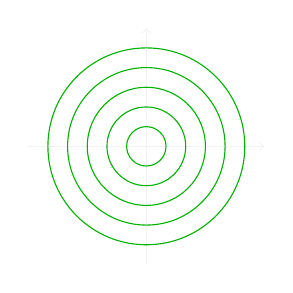
\begin{tikzpicture}[scale=0.5]
      \draw[gray!10,->] (-3,0) -- (3,0);
      \draw[gray!10,->] (0,-3) -- (0,3);
      % family of circles 
      \foreach \r in {0.5,1,1.5,2,2.5}{
        \draw[green!70!black] (0,0) circle (\r);
      }
    \end{tikzpicture}
  \end{center}
  \caption{foliations in \cref{eg:foliation_by_conics} with $a=b$ (left) and $a=-b$ (right).}
  \label{fig:foliation_by_conic}
\end{figure}

\begin{example}
    Let $M = (\bbR / \bbZ)^2$.
  On its universal cover $\bbR^2$, we fix a coordinate $x,y$.
  Let $\tilde{D} = a \partial_x + b \partial_y$.
  It is translation invariant and hence descends to a vector field $D$ on $M$.

  We get two foliation $\tilde{\calF}$ on $\tilde{M}$ generated by $\tilde{D}$ and $\calF$ on $M$ generated by $D$.
  Then leaves of $\calF$ on $M$ are image of leaves of $\tilde{\calF}$ under $\pi: \tilde{M} \to M$.
  Let $L_0$, $\tilde{L_0}$ be leaves through $0$.

  In case $a / b \in \bbQ$, we get a closed loop in $M$.
  Otherwise, we get a dense curve in $M$.
  And hence it is not closed in $M$.
\end{example}


\subsection{Complex settings}

Let $M$ be a complex manifold of complex dimension $m$.
We can define \emph{holomorphic foliations} on $M$ by replacing "smooth" with "holomorphic" and "unit interval" with "unit disk".
The Frobenius theorem (\cref{thm:Frobenius}) also holds in this setting.

\begin{example}
  Let $M = E_1 \times E_2$ where $E_1$, $E_2$ are elliptic curves.
  Write $E_i = \bbC / \Lambda_i$ for $i = 1, 2$.
  Let $D_i \in \Gamma(E_i, \calT_{E_i})$ be a nonzero vector field for $i = 1, 2$.
  Take $D = a p_1^* D_1 + b p_2^* D_2$ for some nonzero constant $a, b$ under $\calT_M \cong p_1^* \calT_{E_1} \oplus p_2^* \calT_{E_2}$.

  Then $D$ defines a holomorphic foliation on $M$.
  Let $L_0$ be the leaf through $0$.
  Then $L_0 \subset M$ is "locally" a holomorphic submanifold of $M$.
  The Chow theorem says that $L_0$ is algebraic if and only if $L_0$ is closed in $M$.

  Case 1: $E_1$ is not isogenous to $E_2$.
  Then $L_0$ is never algebraic.
  Otherwise, the algebraicity of $L_0$ implies that it is an elliptic curve, and hence $E_1$ is isogenous to $E_2$ by $L_0$.

  Case 2: $E_1 = E_2 = E$ and $D_1 = D_2 = D_0$.
  If $a / b \in \bbR \setminus \bbQ$, then $L_0$ is dense in $M$ and hence not algebraic.
\end{example}